\chapter{Experiments}

\section{Synthetic data}

The experiments that follow use synthetic data generated from a structural causal model, which is shown in Figure \ref{fig:scm} \todo[size=\small]{To simplify, removing $x_4$, $y$ and $\hat{y}$.}.

\begin{figure}[!htb]
	\centering
	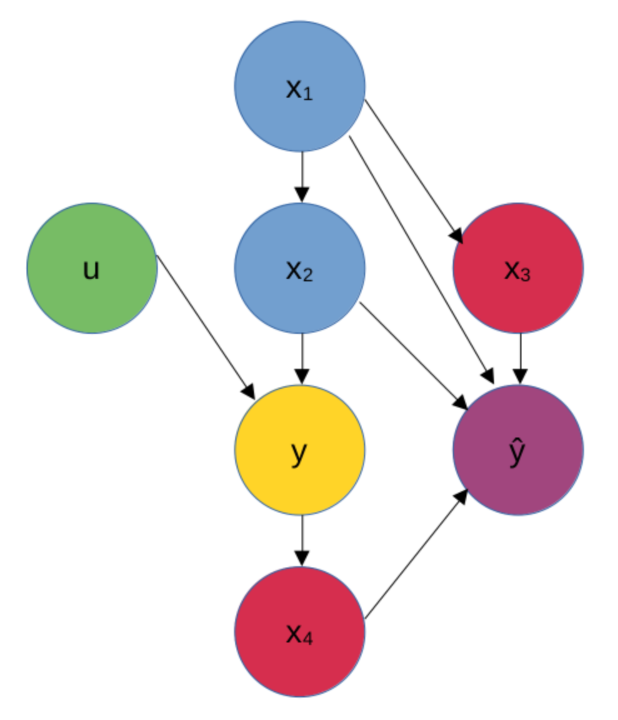
\includegraphics[width=0.4\linewidth]{images/scm.png}
	\caption{The Structural Causal Model used for synthetic data generation}
	\label{fig:scm}
\end{figure}

The structural causal model contains 2 unobserved variables
\begin{itemize}
	\item $\mathbf{u}$ - which is sampled from a normal distribution
	\item $\mathbf{y}$ - the true binary outcome which is a linear combination of $\mathbf{u}$ and $\mathbf{x}_2$
\end{itemize}

And 4 observed variables
\begin{itemize}
	\item $\mathbf{x}_1$ - which is sampled from a normal distribution
	\item $\mathbf{x}_2,\mathbf{x}_3,\mathbf{x}_4$ - which are linear combinations of other variables
	\item $\hat{\mathbf{y}}$ - The predicted value of $\mathbf{y}$
\end{itemize}


\section{Simulation process}

[\textbf{TO CONVERT TO AN ALGORITHM/PSEUDOCODE}]

The process for simulation is as follows. We assume that the individuals do \textit{not} have any knowledge of the classifier.

1. Split the data into test and train sets.

2. Fit a classifier using just the train set and measure accuracy against the *true* labels.

3. Predict labels for \textit{all} data points (both train and test)

4. Calculate recourse actions for all negatively classified data points, by minimising the current approximation of the cost function.

5. Perturb the recourse actions to create pairwise comparisons for the negatively classified individuals to evaluate.

6. Learn cost function from evaluated pairwise comparisons from \textit{all} previous iterations.

7. Generate updated recourse with the current approximation of the cost function.

8. Calculate the 'ground truth cost' of the recourse with learned cost.

\section{Mahalanobis distance}

